\documentclass{article}
\usepackage{amssymb} % Required for math symbols
\usepackage{graphicx} % Required for inserting images
\usepackage[hidelinks]{hyperref}
\usepackage{float}

\usepackage[utf8]{inputenc}
\usepackage{amsmath}
\usepackage[a4paper, total={6in, 10in}]{geometry}
\usepackage{listings}
\usepackage{xcolor}

\definecolor{codegray}{rgb}{0.5,0.5,0.5}
\definecolor{codepurple}{rgb}{0.58,0,0.82}
\definecolor{backcolour}{rgb}{0.95,0.95,0.92}

\lstdefinestyle{cppstyle}{
    backgroundcolor=\color{backcolour},   
    commentstyle=\color{codegray}\ttfamily,
    keywordstyle=\color{blue}\bfseries,
    numberstyle=\tiny\color{gray},
    stringstyle=\color{codepurple},
    basicstyle=\ttfamily\footnotesize,
    breaklines=true,
    captionpos=b,
    keepspaces=true,
    numbers=left,
    numbersep=5pt,
    showspaces=false,
    showstringspaces=false,
    showtabs=false,
    tabsize=2,
    language=C++
}

\title{Laboratorio 2 - Sensores y Actuadores}
\author{jeremy.matos@utec.edu.pe, luis.gutierrez@utec.edu.pe}
\date{Abril 2025}

\begin{document}

\maketitle

\newpage
\tableofcontents
\newpage

\section{Introducción}

\subsection{Objetivo General}

\subsection{Objetivos Específicos}

\newpage

\section{Marco teórico}

\section{Estado del Arte}

% file:///home/tenken/Downloads/30_ShodhKosh_RS_5111.pdf

% https://www.etasr.com/index.php/ETASR/article/view/6410

% https://users.cecs.anu.edu.au/~sid.chau/papers/TOSN-smlight.pdf

% https://www.semanticscholar.org/paper/Innovative-IoT-Smart-Lock-System:-Enhancing-with-Zainuddin-Rahman/563edb5ed5795c9bb35eefc69aa010c9f7c60157

\section{Metodología}

\subsection{SENSORES - Sensor de luz ambiental}

En esta experiencia de laboratorio, se desarrollará un sistema de medición ambiental utilizando los siguientes componentes: 
\begin{itemize}
    \item 1 LDR (sensor de luz)
    \item Diodos LED
    \item Buzzer (alarma)
    \item Botón o switch
\end{itemize}

El objetivo es implementar un sistema que permita medir la cantidad de luz en un ambiente determinado, el cual complementará un sistema de cámaras de seguridad y un control inteligente de luminarias. El sistema debe cumplir con las siguientes funciones:
\begin{enumerate}
    \item Si el nivel de iluminación es bajo, las luminarias de la habitación deben encenderse, representado por el encendido de un LED rojo.
    \item Si el nivel de iluminación es alto, las luminarias deben permanecer apagadas, representado por el LED rojo apagado.
    \item Las cámaras de seguridad deben estar en funcionamiento en todo momento, lo cual se representa mediante el encendido de un LED azul.
    \item En caso de que no se detecte energía eléctrica para el sistema de cámaras (entrada digital detecta GND), el sistema debe encender y apagar el LED azul de manera intermitente, además de activar un buzzer que representa una alarma de error. Esto puede simularse utilizando un botón, un switch o una desconexión de cable.
\end{enumerate}

La implementación se realizó en la plataforma Tinkercad, utilizando un Arduino UNO. La conexión de los componentes se puede observar en la Figura \ref{fig:luz_ambiental}. El sensor LDR se conectó a una entrada analógica (A0), mientras que los LEDs y el buzzer se conectaron a salidas digitales. Un botón se empleó como entrada digital para simular la presencia o ausencia de energía del sistema de cámaras.

\begin{figure}[H]
    \centering
    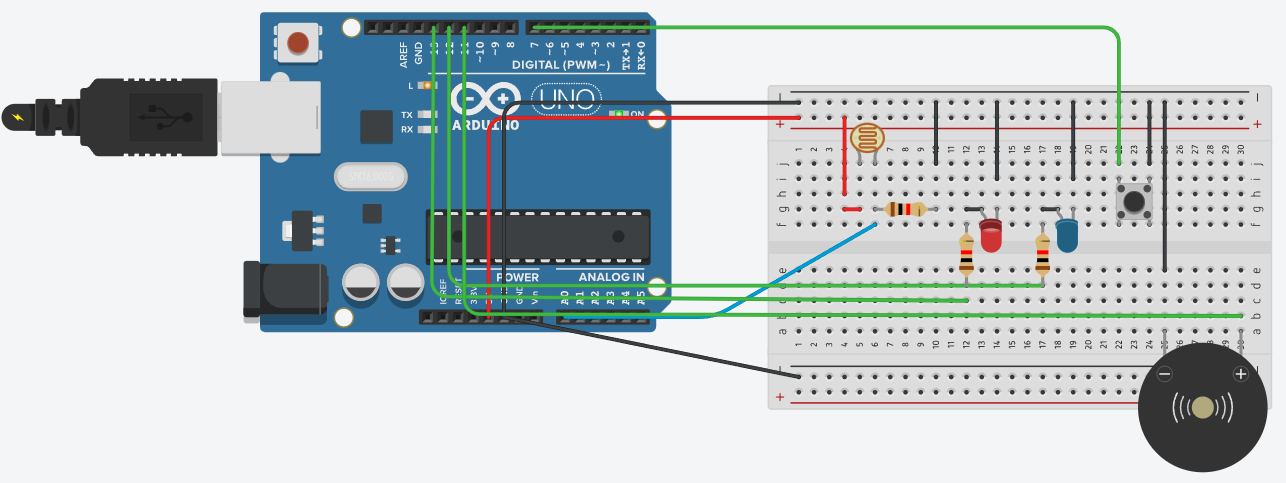
\includegraphics[width=0.85\textwidth]{./img/ckpt_1.png}
    \caption{Simulación Tinkercad Sensor de luz ambiental}
    \label{fig:luz_ambiental}
\end{figure}

En el código (Código \ref{code:sensor_ambiental}), se define un umbral de luminosidad para distinguir entre un ambiente claro u oscuro. Si el valor leído del LDR es menor que este umbral, se activa el LED rojo. Por otro lado, si el botón indica que hay energía (estado HIGH), el LED azul permanece encendido de forma constante. En caso contrario (estado LOW), el sistema simula una falla eléctrica encendiendo el buzzer y haciendo parpadear el LED azul.

\begin{lstlisting}[style=cppstyle, caption={Código en C++ para el sensor ambiental.}, label={code:sensor_ambiental}]
int LDR_pin = A0;
int ROJO_pin = 13;
int AZUL_pin = 12;
int BUZZER_pin = 11;
int BUTTON_pin = 7;
int luz, estadoBoton;
const int umbral = 500;  // Ajustarlo

void setup() {
    pinMode(ROJO_pin, OUTPUT); pinMode(AZUL_pin, OUTPUT);
    pinMode(BUZZER_pin, OUTPUT);
    pinMode(BUTTON_pin, INPUT_PULLUP);
    Serial.begin(9600);
}

void loop() {
    luz = analogRead(LDR_pin);
    estadoBoton = digitalRead(BUTTON_pin);
    Serial.println("Luz: " + String(luz) + " - " + String(umbral));
    
    if (luz < umbral) digitalWrite(ROJO_pin, HIGH);
    else digitalWrite(ROJO_pin, LOW);
    
    if (estadoBoton == HIGH) {
        digitalWrite(AZUL_pin, HIGH);
        digitalWrite(BUZZER_pin, LOW);
    } else {
        digitalWrite(BUZZER_pin, HIGH);
        digitalWrite(AZUL_pin, HIGH); delay(300);
        digitalWrite(AZUL_pin, LOW); delay(300);
    }
    delay(1000);
}    
\end{lstlisting}

\begin{figure}[H]
    \centering
    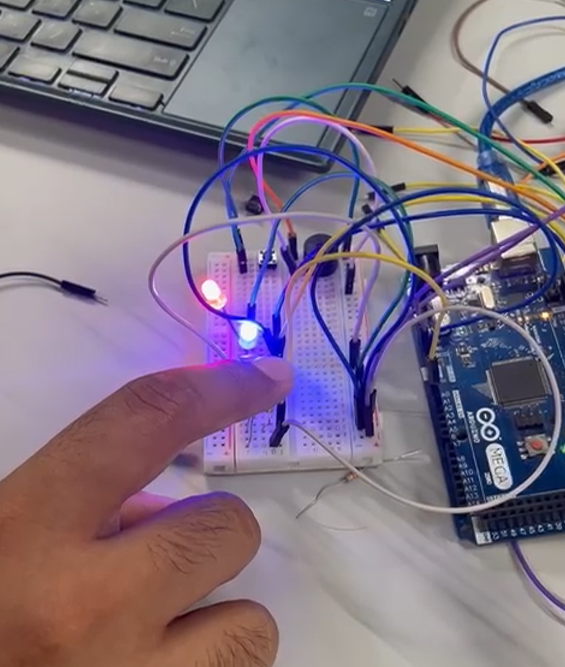
\includegraphics[width=0.85\textwidth]{img/sensores_chkp_2.png}
    \caption{Simulación Tinkercad Sensor de luz ambiental}
    \label{fig:luz_ambiental}
\end{figure}

\begin{figure}[H]
    \centering
    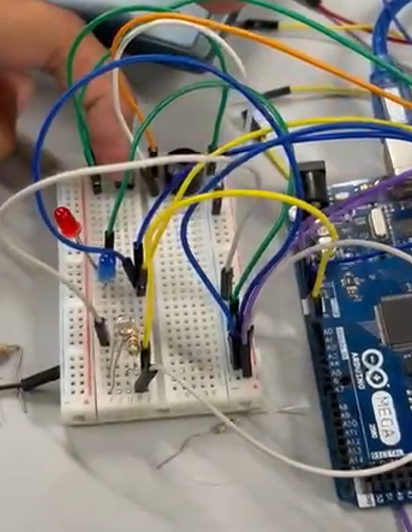
\includegraphics[width=0.85\textwidth]{img/sensores_chkp_2_1.png}
    \caption{Simulación Tinkercad Sensor de luz ambiental}
    \label{fig:luz_ambiental}
\end{figure}

% TODO: foto de la implementacion presencial en el laboratorio

\subsection{SENSORES - Cerradura inteligente}

En esta experiencia de laboratorio, se desarrollará un sistema de seguridad para el control de acceso de personas a un área restringida. Para ello, se utilizarán los siguientes componentes: 

\begin{itemize}
    \item 01 sensor de proximidad.
    \item 01 teclado matricial.
    \item 01 LCD 2x16.
    \item Diodos LED.
    \item Resistencias variadas.
    \item Jumpers.
\end{itemize}

La solución final se puede ver en la Figura \ref{fig:cerradura_smart}. En las siguientes subsecciones se desglosarán las diferentes funcionalidades del sistema.

\begin{figure}[H]
    \centering
    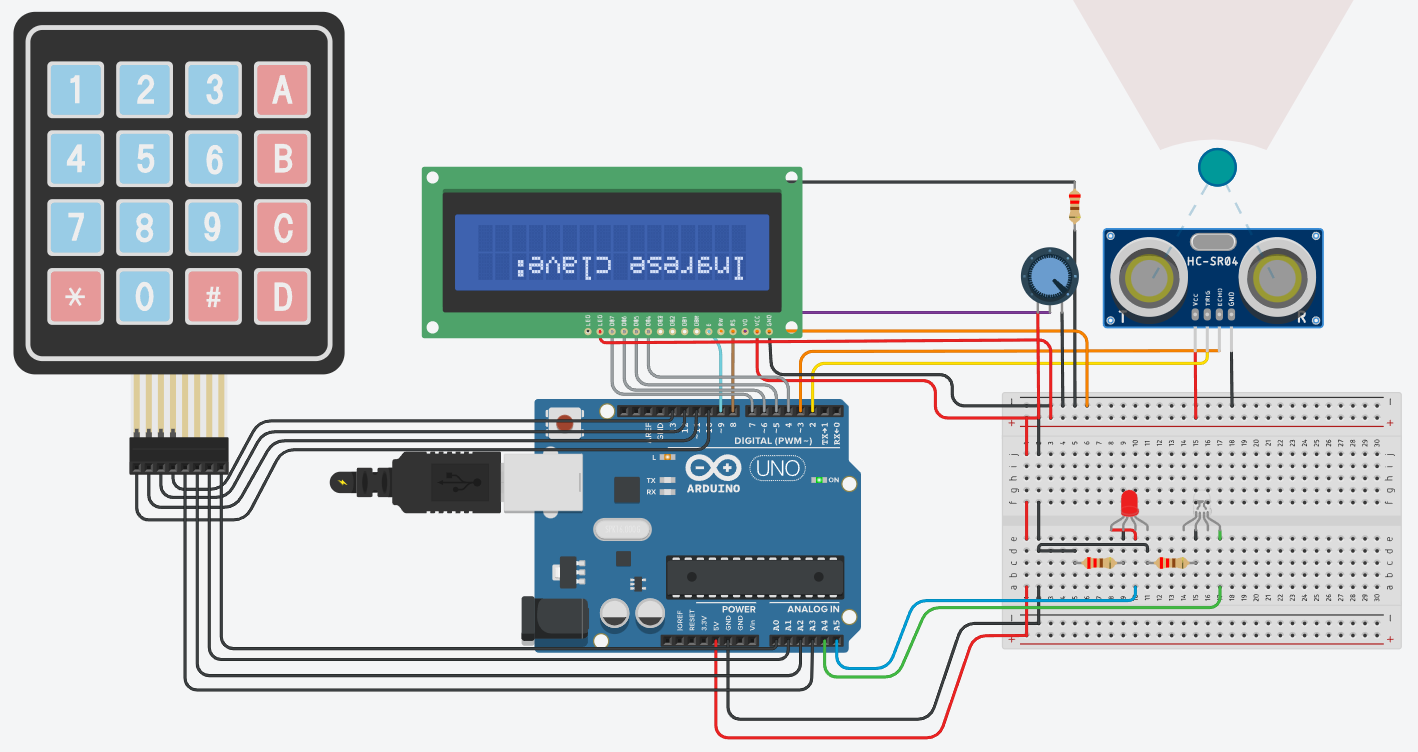
\includegraphics[width=0.85\textwidth]{./img/ckpt_6.png}
    \caption{Simulación Tinkercad Resultado final del sistema de cerradura inteligente}
    \label{fig:cerradura_smart}
\end{figure}

\subsubsection{Presencia de la persona}

\subsubsection{Mensaje en LCD}

\subsubsection{Autenticación}

\subsubsection{Ahorro Energético (Standby)}

\subsection{Sistema de control de aforo}

\begin{figure}[H]
    \centering
    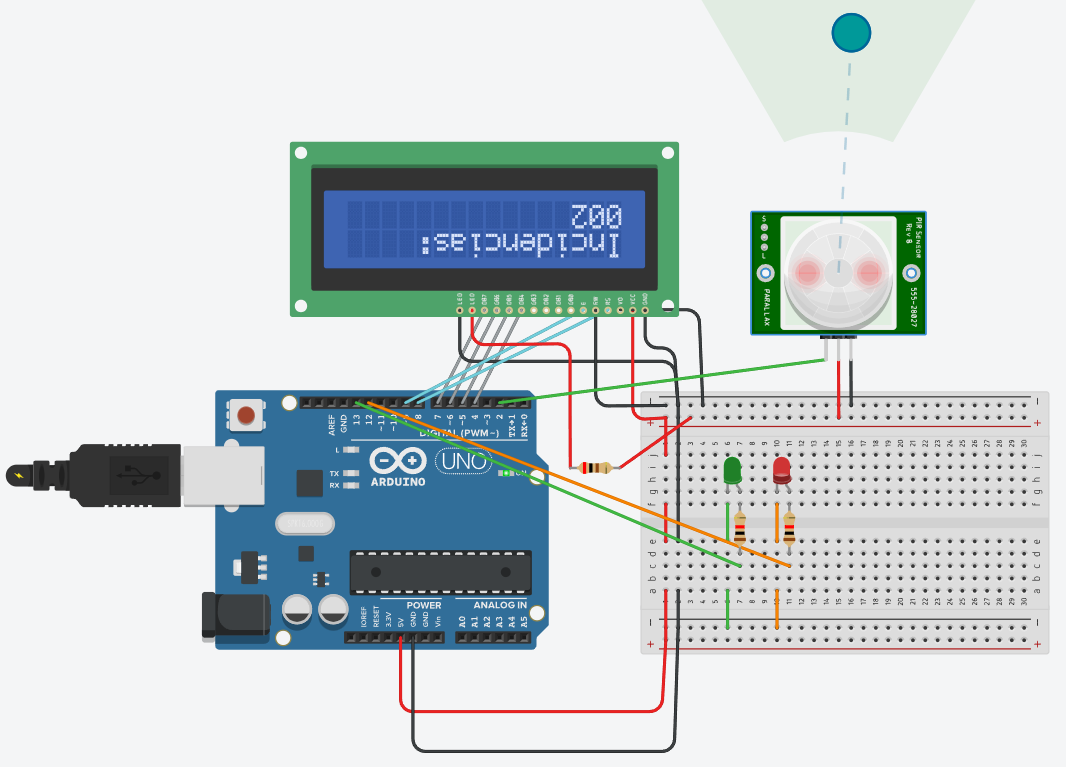
\includegraphics[width=0.85\textwidth]{./img/ckpt_9.png}
    \caption{Simulación Tinkercad Resultado final del sistema de control de aforo}
    \label{fig:control_aforo}
\end{figure}

\begin{lstlisting}[style=cppstyle, caption={Código en C++ para el sistema de control de aforo.}, label={code:sensor_ambiental}]
#include <LiquidCrystal.h>

// Configuracion del LCD
LiquidCrystal lcd(8, 9, 4, 5, 6, 7);
const int PIRPin = 2;
const int LEDGreen = 13;
const int LEDRed = 12;

// Variable to store the number of incidents
int incidentCount = 0;

void setup() {
    Serial.begin(9600);
    
    lcd.begin(16, 2);
    lcd.clear();
    pinMode(PIRPin, INPUT);
    pinMode(LEDGreen, OUTPUT);
    pinMode(LEDRed, OUTPUT);
}

void loop() {
    int value = digitalRead(PIRPin);
    Serial.println(value);

    if (value == LOW) {
    // No movement detected, indicating the rest mode
    digitalWrite(LEDGreen, HIGH);   // Green LED blink (indicates idle state)
    delay(200);
    digitalWrite(LEDGreen, LOW);
    delay(200);
    
    // Display "RESTING" on LCD when no movement detected
    lcd.clear();
    lcd.setCursor(0, 0);
    lcd.print("Modo de Reposo");
    } else {
    // Movement detected, indicating the active state
    digitalWrite(LEDGreen, LOW);    // Turn off the green LED
    digitalWrite(LEDRed, HIGH);     // Turn on the red LED

    // Increment incident count when movement is detected
    incidentCount++;

    // Display incident count on LCD
    lcd.clear();
    lcd.setCursor(0, 0);
    lcd.print("Incidencias: ");
    lcd.setCursor(0, 1);
    lcd.print("00" + String(incidentCount));  // Assuming a 3-digit max count
    
    delay(2000); // Wait 2 seconds before checking again
    }
    
    delay(10);  // Small delay to stabilize the loop
}    
\end{lstlisting}
    
% TODO: diagrama de flujo
% ? TODO: checkpoint 5 y 6 son distintas simulaciones????


\subsection{ACTUADORES - Encendido de un Motor DC con Arduino}

% https://www.tinkercad.com/things/7Ta4Am5NLdF/editel?returnTo=%2Fdashboard%2Fdesigns%2Fcircuits&sharecode=ddM9-NkLnJGgaDXANovwieeo9xofWe2gha9ahUL3Y-o
\begin{figure}[H]
    \centering
    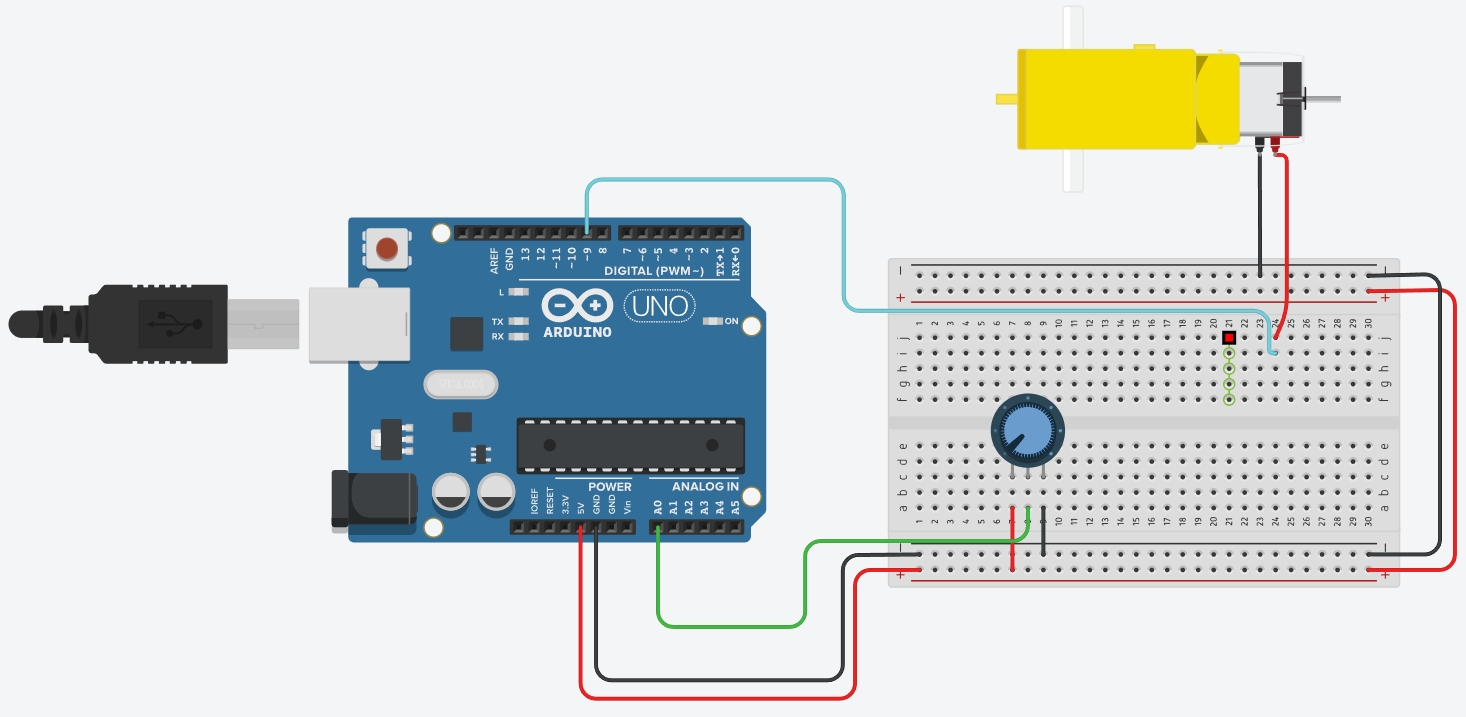
\includegraphics[width=0.85\textwidth]{./img/ckpt_encendido_motor.png}
    \caption{Simulación Tinkercad ...}
    \label{fig:encendido_motor}
\end{figure}


\subsection{ACTUADORES - Control de un motor con Driver}

% https://www.tinkercad.com/things/6vFVydoth82/editel?returnTo=%2Fdashboard%2Fdesigns%2Fcircuits&sharecode=zm5Em3SqUbJ5xXMONP0ul2aEuINO3AnNjSSn-egeFUc

\begin{figure}[H]
    \centering
    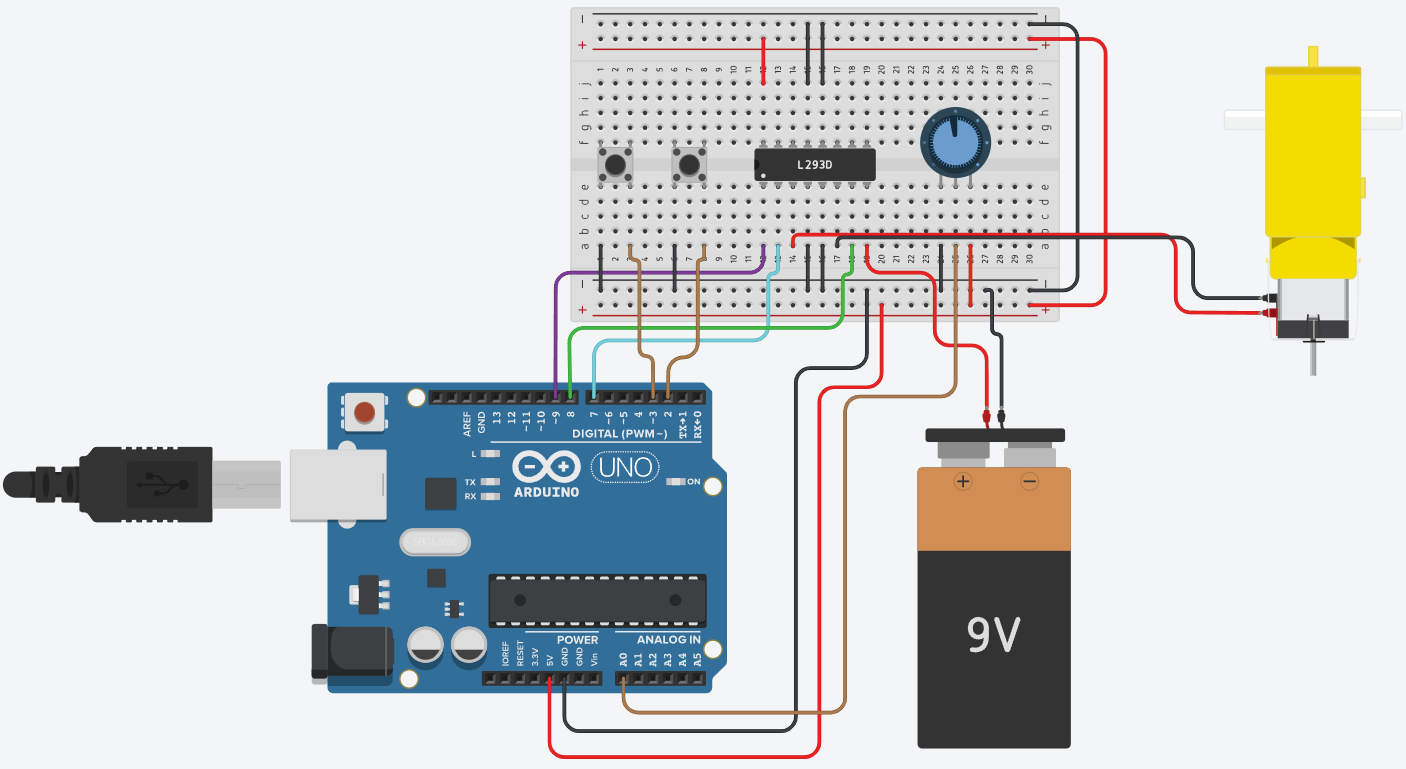
\includegraphics[width=0.85\textwidth]{./img/ckpt_motor_driver.png}
    \caption{Simulación Tinkercad ...}
    \label{fig:motor_driver}
\end{figure}


\subsection{ACTUADORES - Uso de Relé con Motor}

\begin{figure}[H]
    \centering
    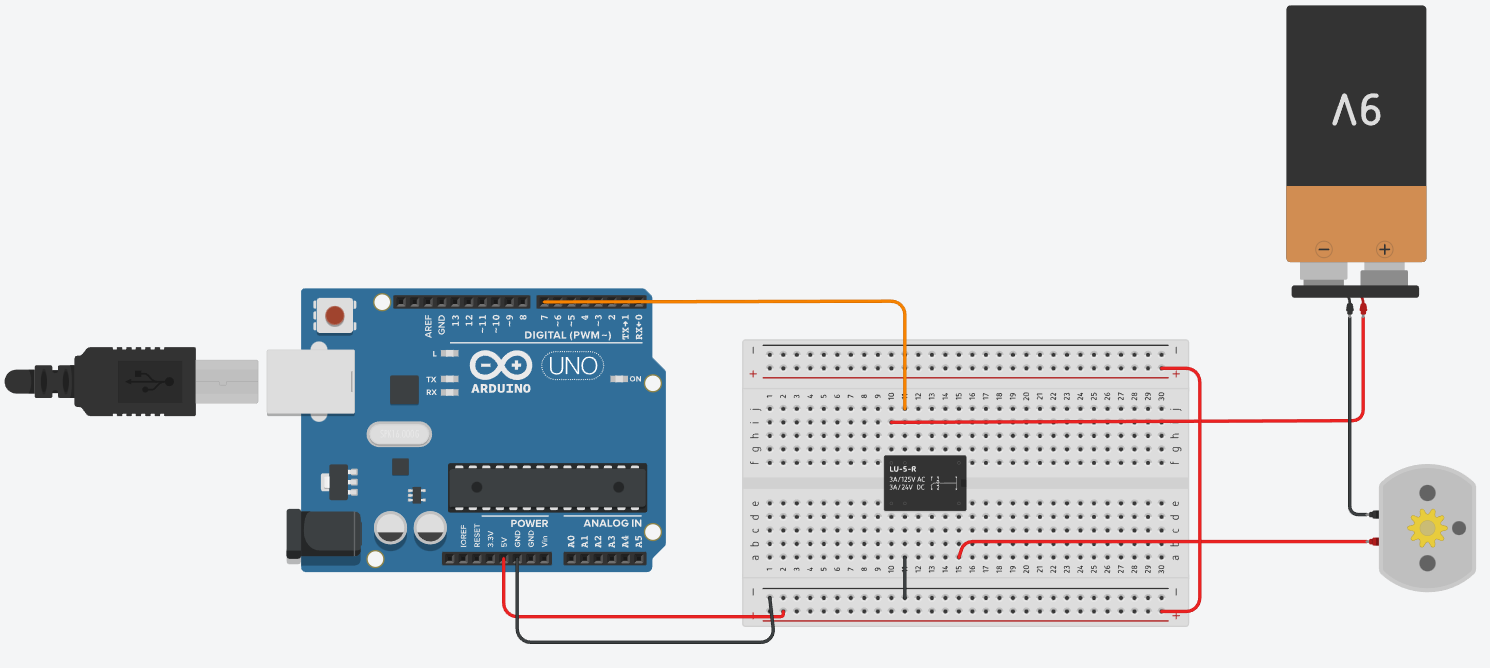
\includegraphics[width=0.85\textwidth]{./img/ckpt_rele_motor.png}
    \caption{Simulación Tinkercad ...}
    \label{fig:motor_driver}
\end{figure}



\section{Conclusiones}

\end{document}
